%     Tokyo Debian Meeting resources
%     Copyright (C) 2011 Junichi Uekawa
%     Copyright (C) 2011 Nobuhiro Iwamatsu
%
%     This program is free software; you can redistribute it and/or modify
%     it under the terms of the GNU General Public License as published by
%     the Free Software Foundation; either version 2 of the License, or
%     (at your option) any later version.
%
%     This program is distributed in the hope that it will be useful,
%     but WITHOUT ANY WARRANTY; without even the implied warreanty of
%     MERCHANTABILITY or FITNESS FOR A PARTICULAR PURPOSE.  See the
%     GNU General Public License for more details.
%
%     You should have received a copy of the GNU General Public License
%     along with this program; if not, write to the Free Software
%     Foundation, Inc., 51 Franklin St, Fifth Floor, Boston, MA  02110-1301 USA

\documentclass[cjk,dvipdfmx,12pt,compress]{beamer}
\usetheme{Tokyo}
\usepackage{monthlypresentation}
\usepackage{moreverb}
\usepackage[varg]{txfonts}
\AtBeginDvi{\special{pdf:tounicode EUC-UCS2}}
% \renewcommand{\familydefault}{\gtdefault}
\renewcommand{\kanjifamilydefault}{\gtdefault}

\title{GPG/PGP キーサインパーティ}
\subtitle{$\sim$ Kansai Open Forum 2012$\sim$}
\author{%
  佐々木洋平/Youhei SASAKI \\%
  \footnotesize{%
    mailto: \texttt{uwabami@debian.or.jp} \\%
    IRC/twitter nick: \texttt{uwabami}}}
\institute{%
  {\footnotesize{keysignparty-ja/Debian JP Project/関西Debian勉強会}}}
\date{%
  {\footnotesize{2012年11月10日 - 於: 大阪南港ATC 10F 特設ステージ}}}
\logo{
\includegraphics[width=3cm]{image201111/logo-gnupg.png}}

\begin{document}

\frame{\titlepage{}}

\begin{frame}{自己紹介}
\begin{itemize}[<+->]

\item 佐々木洋平 (\texttt{@uwabami})
\item Debian JP Project/関西Debian勉強会
  \begin{itemize}
  \item 今日 17:00 から 9F room \#3 で\\
    「Debian 7.0 ``Wheezy''の紹介」 やります.
  \end{itemize}
\item \alert{ksp-ja(key sign party-ja)メンバ}:\\
  \texttt{https://sites.google.com/site/kspjapanese/}
\end{itemize}
\end{frame}

\begin{frame}
\begin{center}
  \huge{なんでキーサインするの?}
\end{center}
\end{frame}

\begin{frame}{なんでキーサインするの?}
  \begin{itemize}[<+->]
  \item PGP/GPG は公開鍵暗号方式
    \\ $\rightarrow$ 公開鍵を誰かに保証してもらう必要がある
  \item しかし PGP/GPG には認証局が無い
    \begin{itemize}
    \item 自分が相手を信頼して、相手が自分を信頼する
    \item これをPGP/GPGユーザで相互に行う
      \\ $\rightarrow$ ネットワークが構築される(\alert{Web of Trust})
    \end{itemize}
  \item 実際に会って、相手の公開鍵と公的ID(パスポート、運転免許証)を確認、そして署名=キーサイン
  \item 誰とも鍵交換してない GPG 署名なんて意味がない
    \\ ...だって誰にも信頼されてないじゃない...
  \end{itemize}
\end{frame}

\begin{frame}{使い所}
\begin{itemize}
  \item 開発者にとっては...
    \begin{itemize}
    \item 存在証明
      \begin{itemize}
      \item 公開サーバのアカウント認証など
      \end{itemize}
    \item ソフトウェアのリリース署名
      \begin{itemize}
      \item Debian、Ubuntu では必須
      \item パッケージへの署名、投票の署名...
      \item Linux カーネル, ...
      \end{itemize}
    \end{itemize}
  \item ユーザによっては...
    \begin{itemize}
    \item メールの署名/暗号化
    \item データファイルの署名
    \item ソフトウェアの改竄チェック
      \begin{itemize}
      \item リポジトリの署名チェック(apt, yum etc..)
      \end{itemize}
    \end{itemize}
  \end{itemize}
  \pause
  \begin{center}
    これらを行うには\alert{Web of Trust}に参加している必要がある
  \end{center}
  \vspace{2.5em}
\end{frame}


\begin{frame}
  \begin{center}
    {\Huge\alert{というわけで、キーサインしましょう。}}
  \end{center}
\end{frame}


\begin{frame}{キーサインの流れ}
\begin{enumerate}
  \item キーサーバに自分の公開鍵をアップロード
  \item 相手の確認(名前、公開鍵の指紋, ID、メールアドレス)
  \item 相手の公開鍵に署名(メールアドレス毎に!)
  \item 署名した相手に公開鍵を送信(メールアドレス毎に!)
  \item 相手に署名された自分の鍵を取り込む
  \item キーサーバに自分の公開鍵をアップロード
\end{enumerate}
\end{frame}

\begin{frame}{キーサインパーティ前のWoT}
\begin{center}
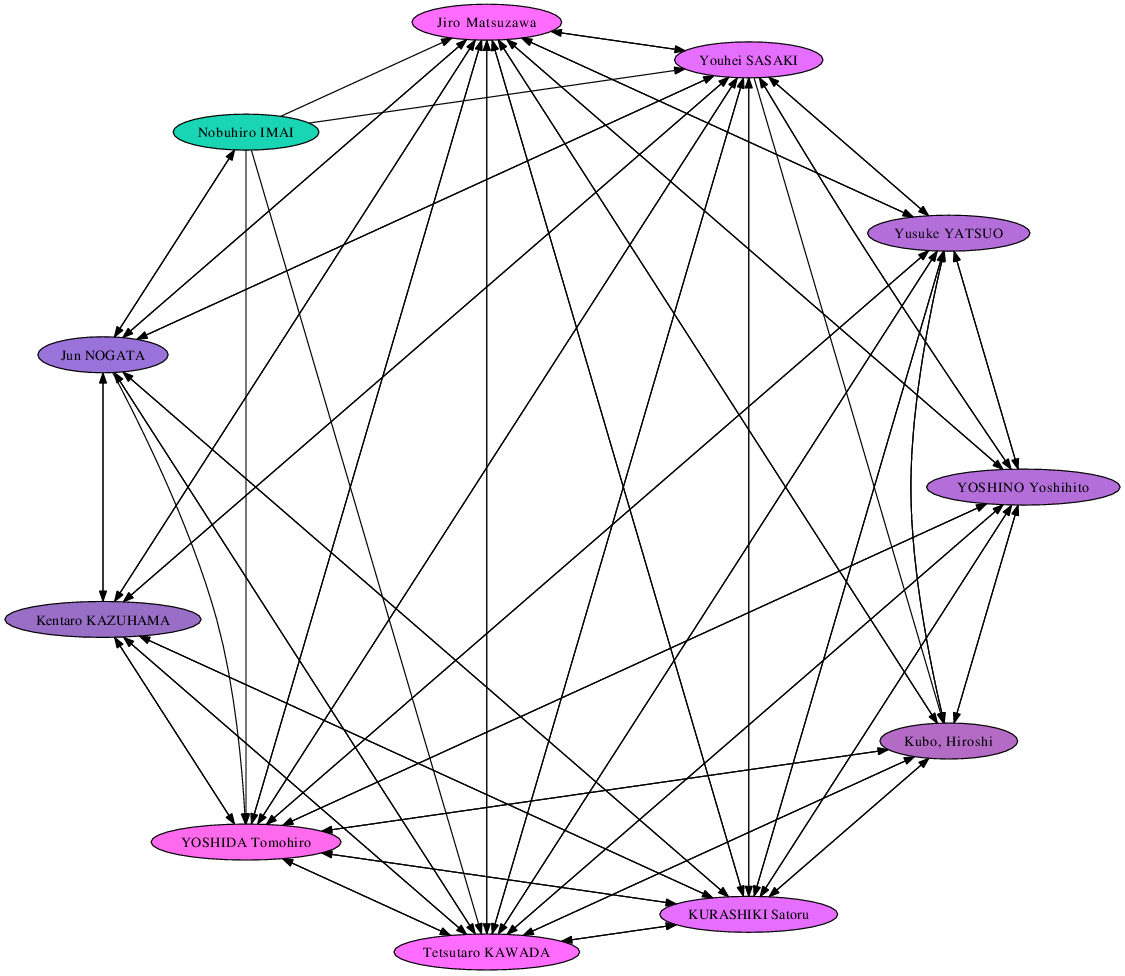
\includegraphics[width=0.8\hsize]{image201211/ksp-before.png}
\end{center}
\end{frame}


\begin{frame}{キーサインパーティ後のWoT (予想)}
\begin{center}
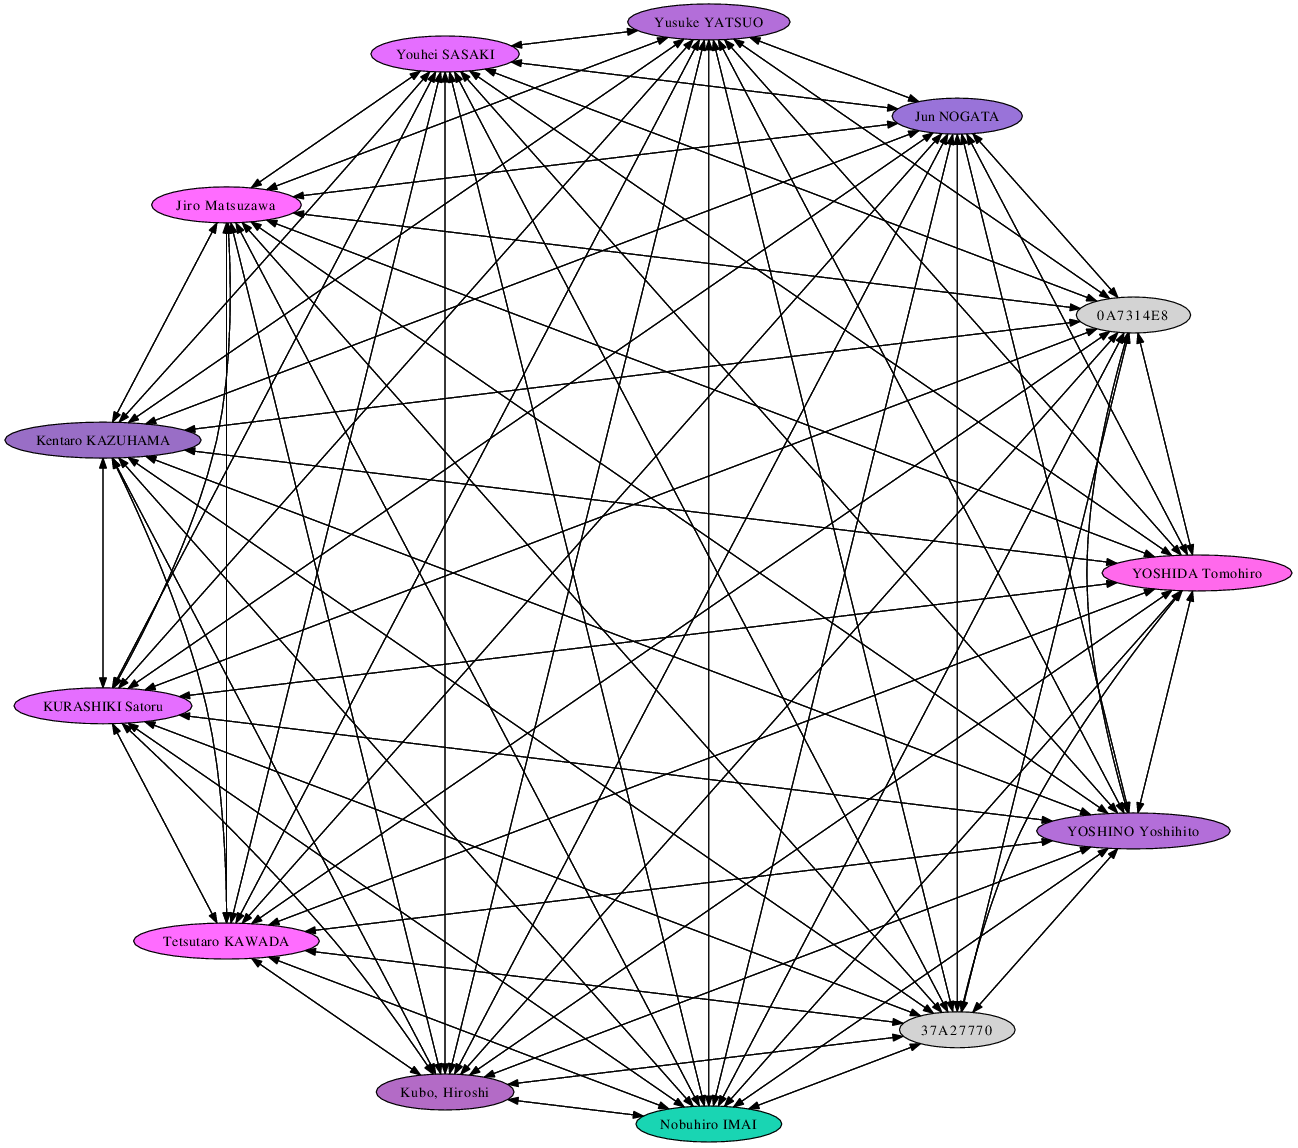
\includegraphics[width=0.8\hsize]{image201211/ksp-after.png}
\end{center}
\end{frame}

\begin{frame}{GPG サインパーティ後}

  \begin{itemize}
  \item 相手にサインして送るまでがGPGサイン。
  \item \alert{caff}を使うと楽ちんです。
  \end{itemize}

\end{frame}

\begin{frame}
  \begin{center}
    {\Huge{Have any questions?}}
  \end{center}
\end{frame}

\begin{frame}{本日の SHA256 ハッシュ}
  \begin{center}
    {\Huge{
        \texttt{05ad 8a0d 63ad f630}\\%
        \texttt{4fb8 61be f4b4 b201}\\%
        \texttt{2776 701c e429 6c2d}\\%
        \texttt{d27e 3375 67b3 8e8c}\\%
      }}
  \end{center}
\end{frame}

\end{document}
